\documentclass{standalone}
\usepackage{tikz}
\usetikzlibrary{patterns, positioning}

\begin{document}
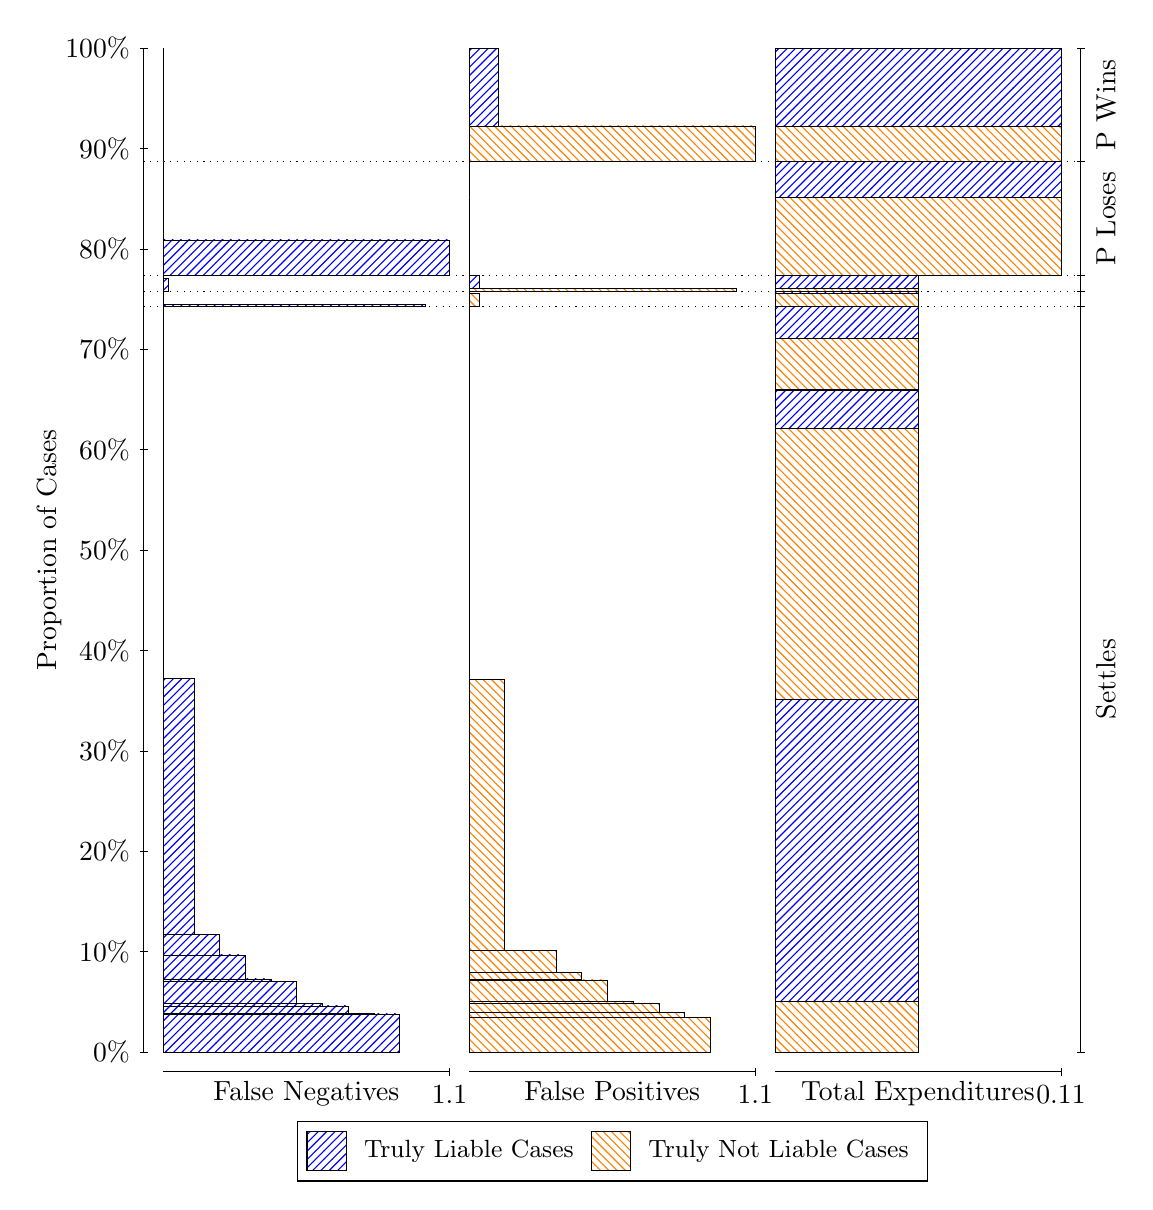
\begin{tikzpicture}
\draw[black, very thin] (1.5,1.75) -- (1.5,14.5);
\node[rotate=90, anchor=center] at (0.3, 8.125) {Proportion of Cases};
\draw[black, very thin] (1.45,1.75) -- (1.55,1.75);
\node[anchor=east] at (1.45, 1.75) {0\%};
\draw[black, very thin] (1.45,3.025) -- (1.55,3.025);
\node[anchor=east] at (1.45, 3.025) {10\%};
\draw[black, very thin] (1.45,4.3) -- (1.55,4.3);
\node[anchor=east] at (1.45, 4.3) {20\%};
\draw[black, very thin] (1.45,5.575) -- (1.55,5.575);
\node[anchor=east] at (1.45, 5.575) {30\%};
\draw[black, very thin] (1.45,6.85) -- (1.55,6.85);
\node[anchor=east] at (1.45, 6.85) {40\%};
\draw[black, very thin] (1.45,8.125) -- (1.55,8.125);
\node[anchor=east] at (1.45, 8.125) {50\%};
\draw[black, very thin] (1.45,9.4) -- (1.55,9.4);
\node[anchor=east] at (1.45, 9.4) {60\%};
\draw[black, very thin] (1.45,10.675) -- (1.55,10.675);
\node[anchor=east] at (1.45, 10.675) {70\%};
\draw[black, very thin] (1.45,11.95) -- (1.55,11.95);
\node[anchor=east] at (1.45, 11.95) {80\%};
\draw[black, very thin] (1.45,13.225) -- (1.55,13.225);
\node[anchor=east] at (1.45, 13.225) {90\%};
\draw[black, very thin] (1.45,14.5) -- (1.55,14.5);
\node[anchor=east] at (1.45, 14.5) {100\%};

\draw[black, very thin] (13.4,1.75) -- (13.4,14.5);
\draw[black, very thin] (13.35,1.75) -- (13.45,1.75);
\node[anchor=west] at (13.35, 1.75) {};
\draw[black, very thin] (13.35,11.22) -- (13.45,11.22);
\node[anchor=west] at (13.35, 11.22) {};
\draw[black, very thin] (13.35,11.411) -- (13.45,11.411);
\node[anchor=west] at (13.35, 11.411) {};
\draw[black, very thin] (13.35,11.611) -- (13.45,11.611);
\node[anchor=west] at (13.35, 11.611) {};
\draw[black, very thin] (13.35,13.057) -- (13.45,13.057);
\node[anchor=west] at (13.35, 13.057) {};
\draw[black, very thin] (13.35,14.5) -- (13.45,14.5);
\node[anchor=west] at (13.35, 14.5) {};

\draw[black, very thin, pattern color=blue, pattern=north east lines] (1.75,1.75) rectangle (4.7506,2.2338);
\draw[black, very thin, pattern color=blue, pattern=north east lines] (1.75,2.2338) rectangle (4.424,2.2368);
\draw[black, very thin, pattern color=blue, pattern=north east lines] (1.75,2.2368) rectangle (4.0974,2.3345);
\draw[black, very thin, pattern color=blue, pattern=north east lines] (1.75,2.3345) rectangle (3.7708,2.3708);
\draw[black, very thin, pattern color=blue, pattern=north east lines] (1.75,2.3708) rectangle (3.7708,2.372);
\draw[black, very thin, pattern color=blue, pattern=north east lines] (1.75,2.372) rectangle (3.4442,2.6493);
\draw[black, very thin, pattern color=blue, pattern=north east lines] (1.75,2.6493) rectangle (3.1176,2.6783);
\draw[black, very thin, pattern color=blue, pattern=north east lines] (1.75,2.6783) rectangle (2.791,2.9841);
\draw[black, very thin, pattern color=blue, pattern=north east lines] (1.75,2.9841) rectangle (2.4644,3.2434);
\draw[black, very thin, pattern color=blue, pattern=north east lines] (1.75,3.2434) rectangle (2.1378,6.4897);
\draw[black, very thin, pattern color=orange, pattern=north west lines] (1.75,6.4897) rectangle (1.75,11.22);
\draw[black, very thin, pattern color=blue, pattern=north east lines] (1.75,11.22) rectangle (5.0772,11.247);
\draw[black, very thin, pattern color=orange, pattern=north west lines] (1.75,11.247) rectangle (1.75,11.411);
\draw[black, very thin, pattern color=blue, pattern=north east lines] (1.75,11.411) rectangle (1.8112,11.577);
\draw[black, very thin, pattern color=orange, pattern=north west lines] (1.75,11.577) rectangle (1.75,11.611);
\draw[black, very thin, pattern color=blue, pattern=north east lines] (1.75,11.611) rectangle (5.3833,12.064);
\draw[black, very thin, pattern color=orange, pattern=north west lines] (1.75,12.064) rectangle (1.75,13.057);
\draw[black, very thin, pattern color=orange, pattern=north west lines] (1.75,13.057) rectangle (1.75,13.51);
\draw[black, very thin, pattern color=blue, pattern=north east lines] (1.75,13.51) rectangle (1.75,14.5);
\draw[black, very thin, pattern color=orange, pattern=north west lines] (5.6333,1.75) rectangle (8.6951,2.1924);
\draw[black, very thin, pattern color=orange, pattern=north west lines] (5.6333,2.1924) rectangle (8.3685,2.252);
\draw[black, very thin, pattern color=orange, pattern=north west lines] (5.6333,2.252) rectangle (8.0419,2.3645);
\draw[black, very thin, pattern color=orange, pattern=north west lines] (5.6333,2.3645) rectangle (7.7154,2.3902);
\draw[black, very thin, pattern color=orange, pattern=north west lines] (5.6333,2.3902) rectangle (7.3888,2.6657);
\draw[black, very thin, pattern color=orange, pattern=north west lines] (5.6333,2.6657) rectangle (7.0622,2.669);
\draw[black, very thin, pattern color=orange, pattern=north west lines] (5.6333,2.669) rectangle (7.0622,2.7626);
\draw[black, very thin, pattern color=orange, pattern=north west lines] (5.6333,2.7626) rectangle (6.7356,3.0371);
\draw[black, very thin, pattern color=orange, pattern=north west lines] (5.6333,3.0371) rectangle (6.409,3.0407);
\draw[black, very thin, pattern color=orange, pattern=north west lines] (5.6333,3.0407) rectangle (6.0824,6.4808);
\draw[black, very thin, pattern color=blue, pattern=north east lines] (5.6333,6.4808) rectangle (5.6333,11.22);
\draw[black, very thin, pattern color=orange, pattern=north west lines] (5.6333,11.22) rectangle (5.7558,11.384);
\draw[black, very thin, pattern color=blue, pattern=north east lines] (5.6333,11.384) rectangle (5.6333,11.411);
\draw[black, very thin, pattern color=orange, pattern=north west lines] (5.6333,11.411) rectangle (9.0217,11.445);
\draw[black, very thin, pattern color=blue, pattern=north east lines] (5.6333,11.445) rectangle (5.7558,11.611);
\draw[black, very thin, pattern color=orange, pattern=north west lines] (5.6333,11.611) rectangle (5.6333,12.604);
\draw[black, very thin, pattern color=blue, pattern=north east lines] (5.6333,12.604) rectangle (5.6333,13.057);
\draw[black, very thin, pattern color=orange, pattern=north west lines] (5.6333,13.057) rectangle (9.2667,13.51);
\draw[black, very thin, pattern color=blue, pattern=north east lines] (5.6333,13.51) rectangle (6.0007,14.5);
\draw[black, very thin, pattern color=orange, pattern=north west lines] (9.5167,1.75) rectangle (11.333,2.3902);
\draw[black, very thin, pattern color=blue, pattern=north east lines] (9.5167,2.3902) rectangle (11.333,6.2306);
\draw[black, very thin, pattern color=orange, pattern=north west lines] (9.5167,6.2306) rectangle (11.333,9.6706);
\draw[black, very thin, pattern color=blue, pattern=north east lines] (9.5167,9.6706) rectangle (11.333,10.154);
\draw[black, very thin, pattern color=orange, pattern=north west lines] (9.5167,10.154) rectangle (11.333,10.158);
\draw[black, very thin, pattern color=blue, pattern=north east lines] (9.5167,10.158) rectangle (11.333,10.161);
\draw[black, very thin, pattern color=orange, pattern=north west lines] (9.5167,10.161) rectangle (11.333,10.808);
\draw[black, very thin, pattern color=blue, pattern=north east lines] (9.5167,10.808) rectangle (11.333,11.22);
\draw[black, very thin, pattern color=orange, pattern=north west lines] (9.5167,11.22) rectangle (11.333,11.384);
\draw[black, very thin, pattern color=blue, pattern=north east lines] (9.5167,11.384) rectangle (11.333,11.411);
\draw[black, very thin, pattern color=orange, pattern=north west lines] (9.5167,11.411) rectangle (11.333,11.445);
\draw[black, very thin, pattern color=blue, pattern=north east lines] (9.5167,11.445) rectangle (11.333,11.611);
\draw[black, very thin, pattern color=orange, pattern=north west lines] (9.5167,11.611) rectangle (13.15,12.604);
\draw[black, very thin, pattern color=blue, pattern=north east lines] (9.5167,12.604) rectangle (13.15,13.057);
\draw[black, very thin, pattern color=orange, pattern=north west lines] (9.5167,13.057) rectangle (13.15,13.51);
\draw[black, very thin, pattern color=blue, pattern=north east lines] (9.5167,13.51) rectangle (13.15,14.5);
\draw[black, dotted] (1.5,11.22) -- (13.4,11.22);
\draw[black, dotted] (1.5,11.411) -- (13.4,11.411);
\draw[black, dotted] (1.5,11.611) -- (13.4,11.611);
\draw[black, dotted] (1.5,13.057) -- (13.4,13.057);
\draw[black, very thin] (1.75,1.5) -- (5.3833,1.5);
\node[anchor=north] at (3.5667, 1.5) {False Negatives};
\draw[black, very thin] (5.3833,1.45) -- (5.3833,1.55);
\node[anchor=north] at (5.3833, 1.45) {1.1};

\draw[black, very thin] (5.6333,1.5) -- (9.2667,1.5);
\node[anchor=north] at (7.45, 1.5) {False Positives};
\draw[black, very thin] (9.2667,1.45) -- (9.2667,1.55);
\node[anchor=north] at (9.2667, 1.45) {1.1};

\draw[black, very thin] (9.5167,1.5) -- (13.15,1.5);
\node[anchor=north] at (11.333, 1.5) {Total Expenditures};
\draw[black, very thin] (13.15,1.45) -- (13.15,1.55);
\node[anchor=north] at (13.15, 1.45) {0.11};

\node[black, centered, rotate=90] at (13.72, 6.4852) {Settles};


\node[black, centered, rotate=90] at (13.72, 12.334) {P Loses};
\node[black, centered, rotate=90] at (13.72, 13.778) {P Wins};

\draw (7.449999999999999,1.5) node[draw=none] (baseCoordinate) {};
\begin{scope}[align=center]
        \matrix[scale=0.5, draw=black, below=0.5cm of baseCoordinate, nodes={draw}, column sep=0.1cm]{
            \node[rectangle, draw, minimum width=0.5cm, minimum height=0.5cm, pattern=north east lines, pattern color=blue] {}; &
            \node[draw=none, font=\small] (B) {Truly Liable Cases}; &
            \node[rectangle, draw, minimum width=0.5cm, minimum height=0.5cm, pattern=north west lines, pattern color=orange] {}; &
            \node[draw=none, font=\small] (B) {Truly Not Liable Cases}; \\
            };
\end{scope}

\end{tikzpicture}
\end{document}